\section{Higgs Reconstruction}

A key ingredient of the analysis is the reconstruction of the two Higgs bosons form the decay of the Higgsinos.
Since this analysis targets events where both Higgs bosons decay to a $b\bar{b}$ pair, the reconstruction starts 
from four jets, which are chosen according to an ordering criterion that favors b-tagged jets over non-tagged jets,
and then orders based on \pt. Practically, this results in the following criteria:
\begin{itemize}
\item If there are exactly four b-tagged jets in the event, those are used.
\item If there are more than four b-tagged jets, the selected ones are the four b-tagged jest with highest \pt.
\item If there are less than four b-tagged jets, the selected ones are the b-tagged ones and the non-tagged ones with highest \pt.
\end{itemize} 

Once the four jets have been selected, they are grouped in two pairs, each one constituting a candidate Higgs bosons. 
Different algorithms to pair the jets have been tested, and the chosen one is based on minimizing the angular separation 
between the two jets associated to the same Higgs boson candidate. 
In particular, the permutation chosen is the one that minimizes:
\begin{equation}
\dRmax = \mathrm{max}(\Delta R(h_1), \Delta R(h_2)) \; ,
\end{equation}

\noindent where $\Delta R(h)$ is the distance in the $\eta-\phi$ space between the two jest from the same candidate.
This choice has a good efficiency in reconstructing the Higgs bosons in the signal, 
and at the same time avoids creating artificial peaks in the background in correspondence of the Higgs boson mass. 


\section{Discriminating Variables}

In this section we show how the variables defined in Section \ref{sec:common_variables} and the ones related
to the Higgs boson reconstruction (\dRmax defined in the previous section, and the mass of the reconstructed Higgs boson candidates)
allow to identify a region of the phase space that is enriched in signal events. 
This study is performed after selecting events with high \met ($> 200$ GeV), at least four signal jets and, least three b-tagged jets, zero signal leptons and \dphimin $>0.4$.
with at least one signal lepton.

Figures \ref{fig:strong:sig:bjets_n} to \ref{fig:strong:sig:met} show the distribution of some important kinematic variables for 
the sum of the \gls{sm} backgrounds and for selected signal samples. 


\section{Signal Regions}

\begin{figure}[htbp]
	\centering
	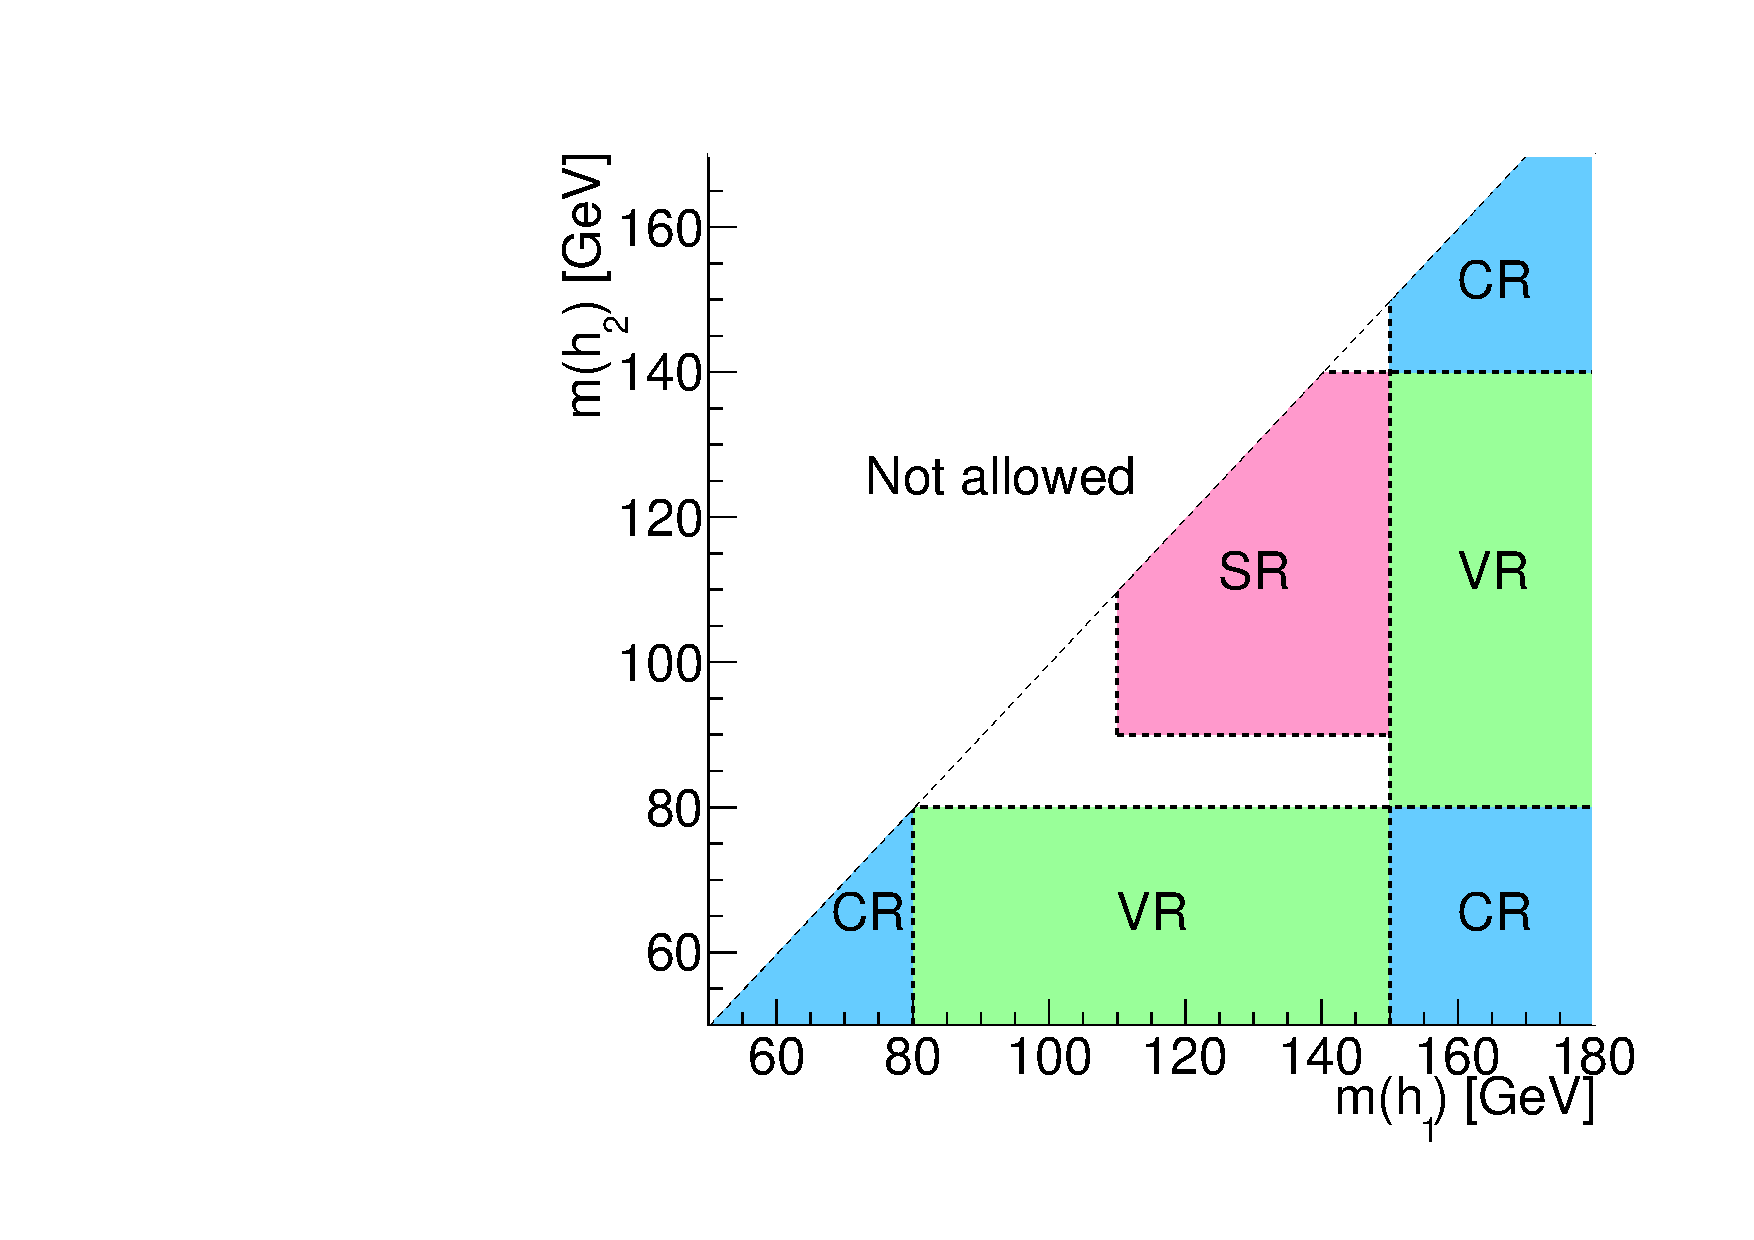
\includegraphics[width=0.490\textwidth]{figures/ewk_prod/varie/schema-1}
	\caption{The division of signal, control, and validation regions using the $m(h_1)$ and $m(h_2)$ variables in the high-mass analysis.}
	\label{fig:binning_crvr}
\end{figure}

\begin{table}[h]
\caption{Signal region definitions for the high-mass analysis. The units of \met, \mtb, $m(h_1)$, $m(h_2)$, and \meffb are GeV. These variables are defined in Section~\ref{high_event_selection}.}
\begin{center}
\resizebox{1.\textwidth}{!}{
\begin{tabular}{|l|c|c|c|c|c|c|c|c|}
\hline
  & SR-3b-meff1-A & SR-3b-meff2-A & SR-3b-meff3-A & SR-4b-meff1-A & SR-4b-meff1-B & SR-4b-meff2-A & SR-4b-meff2-B  & SR-4b-meff1-A-disc \\
 \hline
\nbjet &  $=$3 &  $=$3 &  $\geq$3 &  $\geq$4 &  $\geq$4 &  $\geq$4 &  $\geq$4  & $\geq4$\\
 \hline
\met & \multicolumn{8}{|c|}{$>$ 200}\\
\hline
\dphimin    & \multicolumn{8}{|c|}{$>$0.4}\\
 \hline
\njet &  4--5 &  4--5 &  4--5 &  4--5 &  4--5 &  4--6 &  4--6 & 4--5\\
 \hline
\mtb &  $>$150 &  $>$150 &  $>$130 & - & - & - & - & - \\
 \hline
$m(h_1)$ &    \multicolumn{8}{|c|}{110--150}\\
 \hline
$m(h_2)$ &    \multicolumn{8}{|c|}{90--140}\\
 \hline
\dRmax &  0.4--1.4 &  0.4--1.4 &  0.4--1.4 &  0.4--1.4 &  1.4--2.4 &  0.4--1.4 &  1.4--2.4 & 0.4--1.4 \\
 \hline
\meffb &  600--850 &  850--1100 &  $>$1100 &  600--850 &  600--850 &  850--1100 &  850--1100 & $>600$ \\
 \hline
\end{tabular} 
}

\label{tab:SR}
\end{center}
\end{table}

\section{Control and validation regions}

\begin{table}[h]
\caption{Control region definitions in the high-mass analysis. The units of \met, \mtb, $m(h_1)$, $m(h_2)$, and \meffb are GeV. These variables are defined in Section~\ref{high_event_selection}.}
\begin{center}
\resizebox{0.75\textwidth}{!}{
\begin{tabular}{|l|c|c|c|c|c|}
\hline
  & CR-3b-meff1 & CR-3b-meff2 & CR-3b-meff3 & CR-4b-meff1 & CR-4b-meff2 \\
 \hline
\nbjet &  $=$3 &  $=$3 &  $\geq$3 &  $\geq$4 &  $\geq$4 \\
 \hline
\met  & \multicolumn{5}{|c|}{$>$ 200}\\
 \hline
\dphimin  & \multicolumn{5}{|c|}{$>$0.4}\\
 \hline
\njet &  4--5 &  4--5 &  4--5 &  4--5 &  4--6 \\
 \hline
\mtb &  $>$100 &  $>$100 &  $>$100 & - & - \\
 \hline
$m(h_1)$, $m(h_2)$  &  \multicolumn{5}{|c|}{ ($m(h_1)<$80, $m(h_2)<$80) or ($m(h_1)>$150, $m(h_2)<$80) or ($m(h_1)>$150, $m(h_2)>$140)    }\\
 \hline
\dRmax &  0.4--4 &  0.4--4 &  0.4--4 &  0.4--4 &  $\geq$ 0.4 \\
 \hline
\meffb &  600--850 &  850--1100 &  $>$1100 &  600--850 &  850--1100 \\
 \hline
\end{tabular} 
} 
\label{tab:CR}
\end{center}
\end{table}

\begin{table}[h]
\caption{Validation region definitions in the high-mass analysis. The units of \met, \mtb, $m(h_1)$, $m(h_2)$, and \meffb are GeV. These variables are defined in Section~\ref{high_event_selection}.}
\begin{center}
\resizebox{1\textwidth}{!}{
\begin{tabular}{|l|c|c|c|c|c|c|c|}
\hline
  & VR-3b-meff1-A & VR-3b-meff2-A & VR-3b-meff3-A & VR-4b-meff1-A & VR-4b-meff1-B & VR-4b-meff2-A & VR-4b-meff2-B \\
 \hline
\nbjet &  $=$3 &  $=$3 &  $\geq$3 &  $\geq$4 &  $\geq$4 &  $\geq$4 &  $\geq$4 \\
 \hline
\met  &  \multicolumn{7}{|c|}{$>$200}\\
 \hline
\dphimin &  \multicolumn{7}{|c|}{$>$0.4}\\
 \hline
\njet &  4--5 &  4--5 &  4--5 &  4--5 &  4--5 &  4--6 &  4--6 \\
 \hline
\mtb  & $>$120   & $>$100  & $>$80  & -  &  - & -  & -  \\
 \hline
$m(h_1)$, $m(h_2)$  &  \multicolumn{7}{|c|}{   (80<$m(h_1)$<150, $m(h_2)$<80) or ($m(h_1)$>150, 90<$m(h_2)$<140)   }\\
 \hline
\dRmax &  0.4--1.5 &  0.4--1.7 &  0.4--1.7 &  0.4--1.7 &  1.4--3 &  0.4--1.7 &  1.4--3 \\
 \hline
\meffb   & 550--900   & 800--1150  & $>$1050  & 550--900  & 550--900  & 800--1150  & 800--1150  \\
 \hline
\end{tabular} 
} 
\label{tab:VR}
\end{center}
\end{table}

\section{Pre-fit Data-MC}

The modelling of the main kinematic variables is very similar to what observed in Section \ref{sec:strong:dataMC} 
for the strong-production multi-b analysis, as the few differences in object definitions are not enough to 
lead to a substantial change in data-\gls{mc} agreement; 
this section therefore focuses on the variables specific to Higgs boson reconstruction.
There is nevertheless a notable exception: in the analysis described in this chapter, the data-\gls{mc} agreement in the 
distribution of the number of b-jets is improved, as can be appreciated comparing Figure \ref{} with Figure \ref{}.
This is the result of the 